\documentclass[../main.tex]{subfiles}

\begin{document}

\section{Component Design}

\subsection{Meeple}

The meeple is the component that represents the player's position on the board and provides feedback about player movement, death, and turn roles. It achieves this using two LEDs (a green one and a yellow one) and a hall sensor. Communication with the game controller is facilitated through the MQTT protocol.

The logic governing the meeple is depicted in Figure \ref{fig:meeple-logic}.

\begin{figure}[!htb]
    \centering
    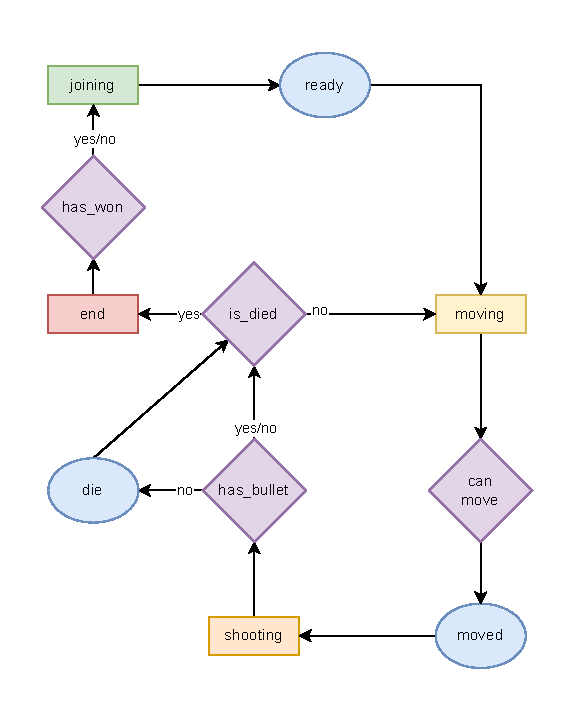
\includegraphics[width=0.7\linewidth]{\subfix{../media/figures/meeple-logic.pdf}}
    \caption{Meeple logic flow diagram}
    \label{fig:meeple-logic}
\end{figure}

Developing the meeple required approximately 10 hours and was completed solely by Christian. While the component was relatively simple to design, my limited experience with electronics and C++ made the process more time-consuming, particularly when trying to create scalable and understandable code.

As mentioned earlier, the most challenging part was ensuring the C++ code worked as intended. Another difficulty was achieving the desired "blinking" effect for the green LED, which required fine-tuning to function properly.

\subsection{Operation base}

The operation base is responsible for determining, when it is its turn, whether the player should shoot or not. Additionally, it provides feedback about the game state through an LCD display, as the operator cannot directly see the game board.

The logic governing the operation base, which relies on MQTT topic subscription and publication, is illustrated in Figure \ref{fig:base-logic}.

\begin{figure}[!htb]
    \centering
    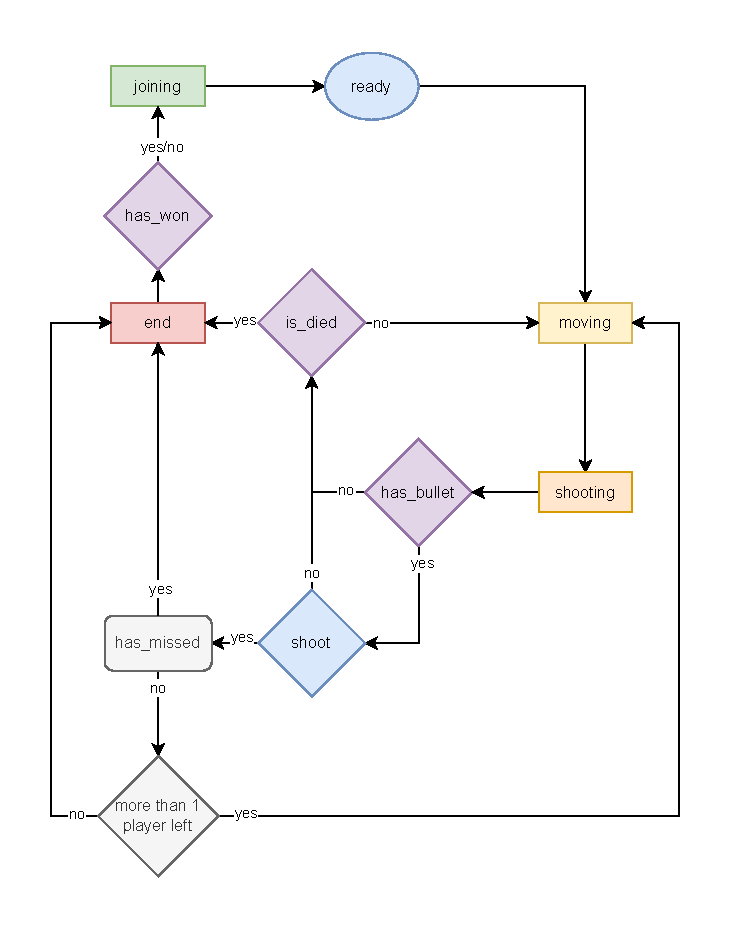
\includegraphics[width=0.8\linewidth]{\subfix{../media/figures/base-logic.pdf}}
    \caption{Operation base logic flow diagram}
    \label{fig:base-logic}
\end{figure}

Developing the operation base required approximately 30 hours and was completed entirely by Jordi.

Initially, all programming was done using Arduino. However, I later migrated most of the code to FreeRTOS. During development, I encountered several challenges. One issue was with the button, which behaved erratically. This was not solely due to switch bounce; interference was also caused by the weak internal pull-up resistor—simply bringing a finger close to the button without touching it affected the readings. Adding an external pull-up resistor resolved this issue.

Another problem involved WiFi connectivity. The ESP32 module was unable to connect to my network. After investigation, I discovered that the ESP32 does not support 5GHz networks, requiring a switch to a 2.4GHz network.

I also faced difficulties connecting to the MQTT broker. The issue stemmed from the broker's IP address changing, but the unclear error messages made diagnosing the problem challenging.

Lastly, I dedicated considerable time to refactoring the code, improving its readability and scalability for future maintenance and enhancements.

\subsection{Game Controller}

The game controller is the core component of the game, responsible for managing the game flow, player turns, game state, and communication with the player feedback system. It operates as a Docker container running a Python script that uses the MQTT protocol in a reactive manner to enable bidirectional communication with the players.

The logic governing the game controller is illustrated in Figure \ref{fig:master-logic}.

\begin{figure}[!htb]
    \centering
    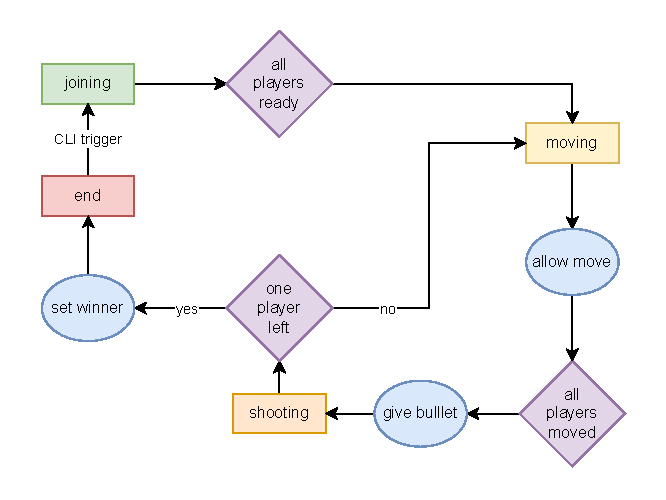
\includegraphics[width=0.8\linewidth]{\subfix{../media/figures/master-logic.pdf}}
    \caption{Master logic flow diagram}
    \label{fig:master-logic}
\end{figure}

Developing the game controller took approximately 20 hours and was completed solely by Christian. We chose Python for the development because it didn’t need to run on a microchip, so performance wasn’t a major concern. Additionally, I’m more familiar with Python, despite having no prior experience with the paho-mqtt library. The most challenging aspect was designing a clean and maintainable project structure. I encountered issues with circular imports while trying to make the code both modular and understandable, and I feel that I struggled with this in some areas.

I developed the meeple and the game controller in parallel, which allowed me to test communication between the two components. While this was beneficial, I was unable to test the game controller with any operation base, so I’m uncertain if it functions as expected in that regard.

\subsection{MQTT Broker}

The MQTT broker is a critical component of the game, enabling seamless communication between all other components. It operates as a Docker container running the Mosquitto MQTT broker.

Developing the MQTT broker required approximately 4 hours and was completed solely by Christian. The most challenging aspect was implementing authentication for the broker. The team also encountered an issue where GitHub altered the line endings in configuration files from LF to CRLF, which caused unexpected failures in the broker's functionality.

Ultimately, Jordi deployed the broker to the cloud, allowing the team to test the game remotely without needing to meet in person

\end{document}